\documentclass[nochapterpage,bigchapter,linedtoc,longdoc,colorback,accentcolor=tud3b]{tudreport}

\usepackage[stable]{footmisc}
\usepackage[ngerman]{hyperref}

\usepackage{longtable}
\usepackage{multirow}
\usepackage{booktabs}

\hypersetup{%
  pdftitle={Making Matches - Recommending the right personality
  },
  pdfauthor={Paul Schweiger},
  pdfsubject={Personality Recommendation},
  pdfview=FitH,
  pdfstartview=FitV
}

\newlength{\longtablewidth}
\setlength{\longtablewidth}{0.7\linewidth}
\addtolength{\longtablewidth}{-\marginparsep}
\addtolength{\longtablewidth}{-\marginparwidth}

\graphicspath{{g/}}


\title{Making Matches - Recommending the right personality}
\subtitle{Paul Schweiger}

\begin{document}
\maketitle

\chapter{Topic Summary}
As globalization and connectedness advance, online communities grow in importance and the offline world embraces online opportunities. A surplus of possible contacts emerges, making it challenging to have an optimal online experience by engaging with fitting personalities. This interaction between users is a cornerstone of many different activities, such as multiplayer gaming, social networks, crowdsourcing communities or online dating platforms, making matchmaking efforts important to further financial and social goals. Recommender Systems that account for an adequate operationalization of the relevant personality traits can be used to improve said goals all across different domains of usage.\\
The ever-growing market of multiplayer gaming experiences have created online spaces where different personalities are forced to work together. While forming an effective team is the apparent goal of competitive online gaming, for the most part of the community \textit{having fun} is even more important. At the same time, the internet's anonymity makes it a great place for trolls and toxic players, resulting in intra-community problems and a “salty” experience. Not only toxic players, but a combination of different player goals and styles can lead to bad experiences: a single aggressive player in a defensive team will not have the needed support in battle, while players aiming for a story-driven experience won’t be able to cooperate with performance-oriented hardcore gamers.\\
Considering the fact that a large amount of players is available at any given moment, it should be possible to incorporate such preferences in the matchmaking process - which is currently mainly driven by player experience and performance. \\
A recent study by Wang et al. \cite{wang2015thinking} looked at the enjoyment of multiplayer sessions in League of Legends (LoL) based on player personality. They followed a subset of Sternberg's \cite{sternberg1999thinking} problem-solving styles in order to categorize the playstyle of different users. While others tried to gain player personality knowledge by simply asking them \cite{riegelsberger2007personality} or other players \cite{patrick2011system}, Wang et al. automated this process with gameplay statistics. They assigned specific in-game actions to each of their player categories and determined a player's style based on his action profile. Choosing the data used to calculate a "good" experience is highly domain specific and depends on available objective game statistics.\cite{delalleau2012beyond} Match enjoyment for LoL was modeled as a function of game length, with shorter games being less enjoyable due to one team dominating the other.  The results show a clear tendency of specific globally-active and risk-taking players to positively influence the overall game enjoyment. A neural network tasked with predicting match enjoyment achieved better scores when player style data was included, suggesting that this might benefit matchmaking algorithms. However, it is important to note that the used measures are highly subjective to LoL, as interviews with players of both LoL and other games confirm.\\
Most Online Dating Services experience comparable problems: Learning who goes good with one another is a major success criterion for dating applications. Possible matchups need to be built according to their preferences rather based upon global performance. Studies predicting user tastes based on the tastes of similar users, a technique called "Collaborative Filtering", showed better results than global matchmaking. \cite{brozovsky2007recommender}\\
Proper personality-based matchmaking in online environments has a positive influence on overall user satisfaction. Successful Recommender Systems need to incorporate personal and detailed data, rather than just performance measurements. On the other hand the limiting effect of Recommender Systems on content diversity needs to be considered, especially in  this social use case. \cite{nguyen2014exploring}\\

\chapter{Introduction}
The modern world has a plethora of opportunities, topics, people, products, and other things, while people have a limited amount of attention and time to spend. In order to help us guide our attention and resources, basically every digital product tries to recommend meaningful content to users. Recommender Systems play a critical role in modern society and have transcended in many different domains.\\
Online communities grow in importance and the offline world embraces online opportunities. A surplus of possible social contacts emerges, making it challenging to engage with the right person at the right time. 
Interaction between users is a cornerstone of many different activities, such as multiplayer gaming, social networks, crowdsourcing communities or online dating platforms. But besides entertainment, social contacts can also further educational goals.\\
SOZIALES LERNEN IST BESSER als Alleine [Quellen]\\
E-Learning and Online Courses -- Wo passt das sinnvoll hin? :S\\
Social Recommendation is more complicated, since it needs to account for preferences of more than just a single person. Recommender Systems need account for an adequate operationalization of the relevant personality traits, domain-specific skills and surrounding circumstances.\\
\\
Focus on E-Learning and Reciprocal Recommendation, because...\\
Introduction to Recommendation in E-Learning (How good is research? Overlap with other topics -> shorten this section)\\
Introduction to Recommendation in Reciprocal environments (How good is this researched? How many things do we know?)\\
This report will discuss possible solutions to improve learning via reciprocal peer recommendation in Learning-Environments. As one of the first (???) and the most recent implementation of such an endeavor, the report will provide a detailed overview of XXXXXXXXX by XXXXXXXX. Important findings leading up towards the work, possible extensions and research in other fields that might prove to be beneficial to this study will be discussed.\\

\chapter{Research leading towards the paper}
\section{Learning}
TODO: Provide overview of modern learning:\\
\begin{itemize}
	\item learner types
	\item E-Learning vs. offline learning
	\item peer learning
	\item recommender systems for e-learning so far
\end{itemize}

\section{Recommender Systems}
TODO: Provide short overview of RS\\
Where do they come from, what have they been used for?\\
REMARK: This section might be removed due to overlap with other sections. Maybe RS for E-Learning and reciprocal RS will be enough\\

\section{Reciprocal Recommendation}
TODO: Provide Overview of Reciprocal Recommendation\\
\begin{itemize}
	\item Goal of recirpocal recommendation
	\item different ways to do this: Just a score for other people, or actual reciprocal recommendations, where bothpartners see each other as a recom.
	\item Other fields (Gaming, Dating)
	\item Common methods (Collaborative Filtering)
	\item Common problems encountered when doing this (operationalize personality / relevant aspects, acquire personal information about people, self-reported vs. implicit, ...)
\end{itemize}

\chapter{Reciprocal Peer Recommendation for Learning Purposes}
\section{Introduction}
Introduction: Motivation for this specific study. What did they want to accomplish?\\
Explain goals and problems of 
XXX et al. implemented RiPPLE to prove their theories. 
\section{RiPPLE}
RiPPLE ["Recommendation in Personalised Peer Learning Environments"] was designed and developed as a web-based prototype online learning recommendation. RiPPLE is an adaptive, student-facing, open-source platform with the aim to enable students to engage with others in meaningful learning experiences. To enhance the learning experience, RiPPLE functions as a learning platform, helping students to co-create and find meaningful learning-content and to find peers to learn with. This analysis will focus on RiPPLE as a peer recommendation platform.\\
Based on user input, RiPPLE will calculate potential matchups for its users. Depending on the competency derived by a user's performance on learning content, his or her available timeslots and a user's preference on the topics and partner's competency he would like to provide or seek peer support or find a learning partner in, RiPPLE calculates a score for a matchup and will recommend a predefined amount of persons to each user. As RiPPLE currently recommends learning opportunities for the upcoming week, updates to user preferences or competencies are represented once per week.\\
An important aspect of the recommendation algorithm is it's compatibility function, calculating a one-directional score for each combination of potential study partners, u1 and u2. In the first step, the algorithm will check whether a potential matchup is viable following two hard constraints:
\begin{itemize}
	\item a shared timeslot has to be available for both u1 and u2
	\item the topic-specific joint competency must be greater than a prefedined threshold T. According to BLUMENFELD [QUELLE], peer learning sessions will only become effective once the learners can share a minimum understanding of the topic.
\end{itemize}
For every pair of users satisfying these constraints, RiPPLE will calculate the user's respective one-directional scores. These represent how fitting u2 is as a study partner for u1 and vice-versa. (Since the users could have defined different preferences for their competency differences, scores don't need to be symmetric.) The scores take into account how good a matchup will be in terms of overall competency level, and how the other user matches the current users preferences. These calculations will be calculated across all topics relevant for u1 and u2.\\
These two one-directional scores (the score of u2 as a partner for u1 and the score of u1 as a partner of u2,) could now be used to find the the best partner for a specific user. To further recommend a matchup that is beneficial for both u1 and u2, the harmonic mean of both scores is considered as the "reciprocal score" of u1 and u2, a value that is now symmetric. [QUELLE PRABKAHAR 45] The harmonic mean, contrary to the arithmetic mean, pays respect to differences between it's values, making a larger gap between values less desirable. Peer-combinations with approximately similar scores in each direction will receive better final values, pushing matchups that are beneficial to both participants more relevant.\\
TODO: BILD VON SCORES; SCORES ALS VERTEILUNGEN\\
In the last step, RiPPLE returns a predefined amount of matchups with the best reciprocal values for each user. Although these reciprocal values are now symmetrical, the recommendations don't have to be: While from u1s standpoint the matchup with u2 and an (arbitrary) reciprocal score of 30 could be the very best opportunity, u2 could still have a matchup with u3 and a value of 50.\\
For more information on RiPPLE, the algorithm and further clarification of different variables, please reference [QUELLE].\\	
RiPPLE will be evaluated in live conditions in the course of this year. To check whether the implementation could work under real conditions, XXXX conducted an evaluation using randomly generated data. This will be discussed in the upcoming section\\

\section{Evaluation}
In order to test RiPPLE's applicability for actual use, Potts et al. designed an experimental setup in which RiPPLE would try to propose recommendations for randomly generated test data. Specific quality measures were designed to assess different fields in which RiPPLE would have to show its capabilities. With satisfying results, RiPPLE would be able to be used under live conditionsin the course of 2018.\\
\\
To conduct the experimental evaluation, random data had to be generated; diverse enough to highlight edge cases but within reasonable bounds. For a set of 1000 users, 10 learning topics and 10 possible timeslots, each user received a random distribution of relevant values. Topic-specific competencies were expressed as a value from 0 to 100 derived from a truncated normal distribution around a random mean with fixed variance. Each user received competencies for every topic. These were then sorted from low to high, and a random number of these topics were chosen to be part of the user's request. The highest competencies of every user were classified as "providing support" roles, the lowest as "seeking support" and the median topic received a "co-study" role. In absence of empirical data, competency difference preferences were modeled as a fixed value per chosen role, as opposed to a explicitly stated preference for each user. Every "user" was made available during random timeslots.\\
\\
To fully satisfy as a tool to recommend students to one another, Ripple must be able to form meaningful and successful matches for as many users as possible in reasonable time. On the other hand, minor drawbacks in the defined metrics were considered to be tolerable due to the experimental and randomly generated data and some further adjustments that could be made to compensate bad values.\\
As Evaluation Metrics for their experimental evaluation Potts et al. decided on four values that can further be used as general Quality Measures for reciprocal recommendation algorithms:\\

\subsection{Scalability} With increasing enrollment numbers in higher education, RiPPLE will have to be suitable for large sets of learners. High runtime and costs for evaluating datasets with reasonable amounts of students means slower responses and a worse user experience. An optimal solution could provide immediate recommendations to any user, at any moment.\\
As can be seen in figure \ref{f:scalability}, the runtime of the algorithm increased in a quadratic fashion, as U, the total amount of users, increased: \(O(n^2)\). The number of recommendations per user, however, does not significantly impact the runtime. (Although the paper states that it \textit{did} in fact affect runtime, looking at the plotted data suggests that this might be a formatting error.)\\
Currently, RiPPLE calculates recommendations at the end of each week for the upcoming week, making the algorithm's runtime rather unimportant. However, further improvements are planned.\\
In a 1000 user experiment, RiPPLE was able to provide recommendations for a single user in 0.045 seconds - which is a pretty good time.\\
\begin{figure}[p]
	\centering
	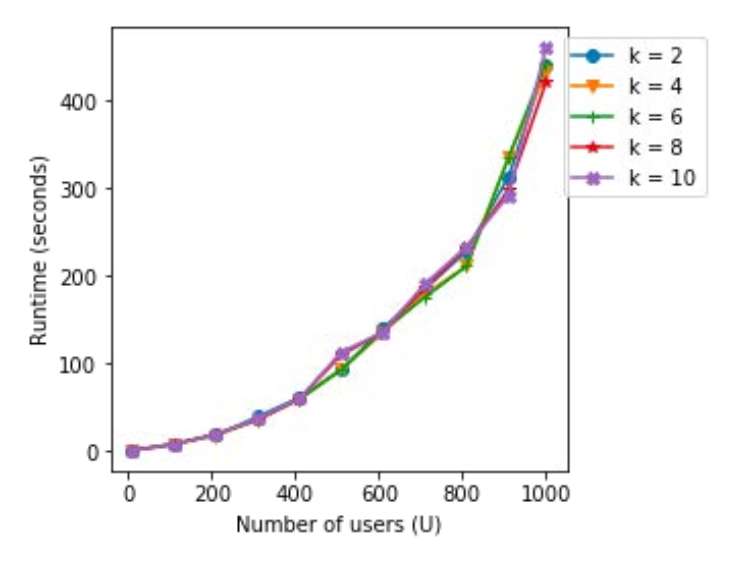
\includegraphics[width=0.5\textwidth]{g/Runtime.PNG}
	\caption{Scalability: The algorithm's runtime depending on the number of users \(U\) and the amount of recommendations per user \(k\). Note how k has almost no influence on the runtime, while it grows exponentially with increasing U. Source: \cite{potts2018reciprocal}}
	\label{f:scalability}
\end{figure}


\subsection{Reciprocality} The best possible recommendations are reciprocal: Users contacting a recommended user would also appear on this user's list of potential study partners. Reciprocality was tested for both, the baseline non-reciprocal and the joint reciprocal average scores. Whenever a user appears in the recommendations of a user on their own recommendation list that was built according to the respective score, the recommendation was considered to be reciprocal.\\
The precision for every user given the used score is calculated by dividing his reciprocal recommendations through \(k\), the total amount of recommendations that user received. The system's total precision is defined as the average precision across all users.\\ 
QUELLE\\
In all tested cases shown in figure \ref{f:reciprocality}, the reciprocal score had a higher precision than the baseline score. This is not surprising, since using the harmonic mean of both one-directional scores chooses reciprocal scores with medium values compared to non-reciprocal scores with a single high value. [REFERENZ AUF ERKLÄRUNGSABSCHNITT] Increasing \(k\) also increases the precision, since more recommendations per user lead to a higher chance of reciprocal recommendations. On the other hand, increasing \(U\) with a fixed \(k\) reduces reciprocal precision, since there are more possible users to recommend.\\
\begin{figure}[p]
	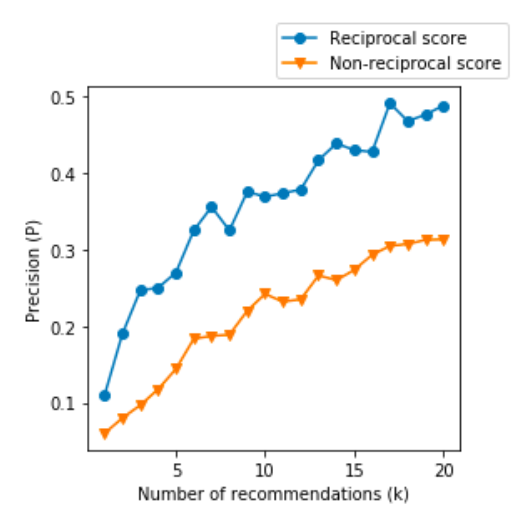
\includegraphics[width=0.5\textwidth]{g/PrecisionByK.PNG}
	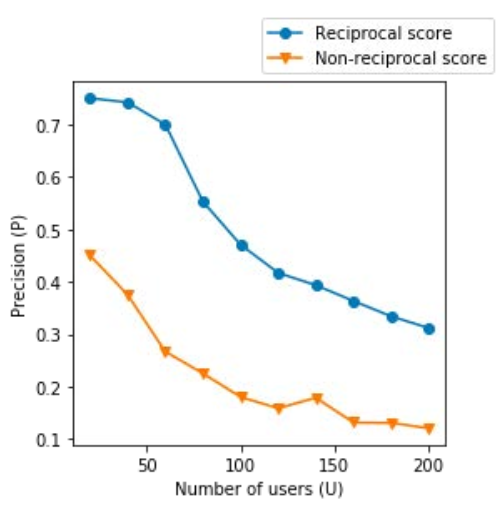
\includegraphics[width=0.5\textwidth]{g/PrecisionByU.PNG}
	\caption{Reciprocality: The precision (= the fraction of reciprocal recommendations out of the total recommendations averaged over all users) of the baseline non-reciprocal recommendations (orange) vs. of the reciprocal, averaged scores. Note how the reciprocal scores are always better. Source: \cite{potts2018reciprocal}}
	\label{f:reciprocality}
\end{figure}

\subsection{Coverage} Recommending potential learning partners to one another should be made for as many users as possible, not abandoning anyone. As such, coverage is a very important metric to consider. Since (almost) every user will receive recommendations, most users will be covered in one way or another. (The exception to this are users with completely incompatible timeslots, role preferences (i.e. being the only person looking for an equally skilled study partner) or users who can't meet the minimum competency when coupled with their available potential partners.) A good fit can only be ensured when the same user is recommended to others, ideally forming a reciprocal recommendation, which is represented in another quality measure. Coverage however is defined as the percentage of users that appear in other's recommendations at least once.\\
For a low amount of users and lots of recommendations per user, coverage is close to 0.9, meaning most users are recommended to others. As U increases or k decreases, the coverage sinks. However, more than 40\% of users appear in other's recommendations under all tested circumstances. Reference figure \ref{f:coverage} for a graphical overview.\\

\begin{figure}[p]
	\includegraphics[width=0.5\textwidth]{g/CoverageUk.PNG}
	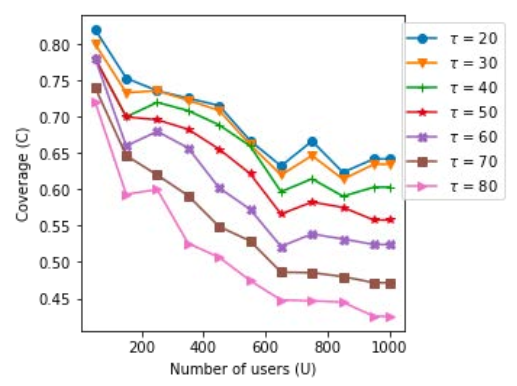
\includegraphics[width=0.5\textwidth]{g/CoverageUT.PNG}
	\caption{Coverage: The percentage of users who appear in other's recommendations. With more users, coverage sinks (likelihood of hard to match users increases). Increasing received recommendations or lowering the minimum joint competency of matches increases coverage. Mind the y-axis cutoff. Source: \cite{potts2018reciprocal}}
	\label{f:coverage}
\end{figure}

\subsection{Quality} The quality of a recommendation is not only based on its fit, but also on how good the resulting team could perform. According to BLUMENFELD QUELLE, learners should meet a minimum competency level in order to be an effective group, as specified by the employed minimum matchup threshold T and leniency factor alpha. [IST ES GUT DIE HIER ZU ERWÄHNEN? HÄNGT DAVON AB WIE ICH DIE BILDER EINBINDE] Quality is thus defined as the user's average joint competencies across their matched topics. The goal is to generate matches, that are as capable as possible in their respective fields of study.\\
Referencing figure \ref{f:quality}, it is apparent that the total amount of users does not affect the quality of matches. The minimum threshold for joint competency of a matchup however leads to a better quality. Comparing this finding to \ref{f:coverage} however, suggests that higher quality comes at the cost of less coverage. Especially when considering the slight improvements in quality score for larger increments in T.\\
\begin{figure}[p]
	\centering
	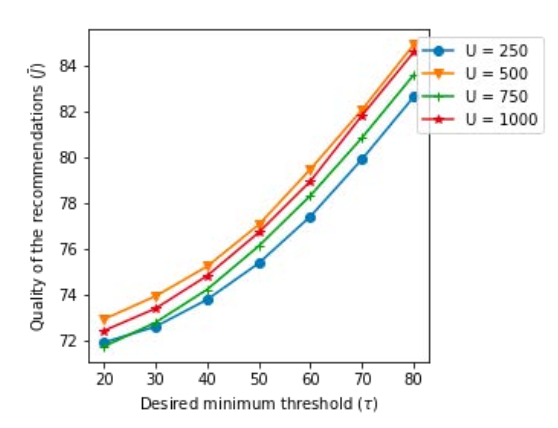
\includegraphics[width=0.5\textwidth]{g/QualityByU.PNG}
	\caption{Quality: The quality of matchups over different values for U and T. Note how changing U won't affect matchup quality. Choosing a higher minimum joint competency threshold T for successful matchups increases overall quality. Note the different scaling of the axes, overemphasizing the quality increases. Source: \cite{potts2018reciprocal}}
	\label{f:quality}
\end{figure}

\section{Discussion}
"Reciprocal peer recommendation for Learning Purposes" and the implemented platform RiPPLE present an approach to build a scalable, interactive and user-facing, multi-purposes learning platform to enhance learning both in on- and offline circumstances. RiPPLE's flexiblity in some threshold values allows the tool to be customised to address some of the shortcomings of peer recommender systems identified by OLAKANMI AND VASSILEVA QUELLE. While the experimental results look promising, further research on actual data has to be conducted, which is planned over the course of the year.\\
Recap of their discussion\\
The experimental evaluation of the platform's performance using artificial data sheds light on variable relationships, potential initial values for scientifically sparse concepts and the interplay of lots of factors. While the values reported from evaluation with artificial data present good metrics to measure the algorithm's performance and suitability for live data, they don't actually evaluate the algorithm, since no targets have been set. Although the data is quantifiable, these findings should not be mistaken as quantitative results: instead of comparing the data to theory-driven goals and evaluating them for actual use, they are more or less providing an overview of how the algorithm works. In fact, there is currently no way to know of these results are "good". \textit{Many of the used measurements lack consistent data and research, and are not theoretically funded.} The question whether a coverage of little above 0.4 will be enough in practice, remains unanswered. Actual results from live usage are thus highly interesting and could provide insights in lots of different areas.\\
\\
The algorithm itself does have some minor drawbacks. For one, RiPPLE calculates matchups across all topics. For example, two learners who would be a perfect match in one topic, but a bad match in another would be considered as a mediocre match. Topic-wise recommendation would further complicate the algorithm, but might lead to larger benefits for users. Edge-cases in terms of competency preferences would lead to overall low scores for matchups with other people, leading to learners who will receive suggestions with low scores, but won't appear in other's recommendations. While this does not necessarily lead to any consequences by itself, certain highly compatible users might be overwhelmed with meating-requests from users outside their own recommendations. While they won't be able to meet every requesting user, these less compatible users might become abandoned.\\

Another drawback is the neglected human factor. Both user buy-in and competence in handling the tool and its demands might influence its use in practice. While this study's goal was explicitly to test the theory and future praxis tests are planned, this topic should be discussed, a major shortcoming of the paper at hand.\\
A lack in user buy-in is something that always should be considered, especially in a student context. If a student didn't want to engage with strangers, was not motivated to study with partners or to adjust his or her schedule, all recommendations to and of that student would not accomplish anything. Meeting requests would be ignored, and opportunities for matchups would expire. Even negative user manipulation needs to be considered as an possibility, but is something that has to be dealt with in the live test.\\
While missed opportunities are a problem of the students themselves, rather than of the platform providing recommendations, the other human factor needs to be addressed directly by the tool:\\
As humans are unreliable, self-reported metrics always underly lots of variance and errors. A user's competency in a specific topic, his or her preferences, or the willingness to commit a specific timeslot to learning might change daily, dependant on mood, time of day and lots of other factors. [QUELLE?] Other variables, like a user's preferred skill difference towards a learning partner, are especially hard to specify. How is a user supposed to know what his or her learning preferences are? How would he know which number refers to the desired difference in skill rating? From a psychological standpoint, this operationalization is bound to fail. [Compare criticism to Likert scaled items QUELLE]\\
All of this taken into consideration, the proposed peer learner recommendation algorithm does have its flaws but will not necessarily fail. The benefits of recommending meaningful social learning opportunities are manifold and even if RiPPLE will only be used by a fraction of the potential users, it will surely help these learners to navigate a digital world full of learning opportunities. The live test will show, whether this hypothesis holds in praxis.\\


\chapter{Extensions}
TODO: Include possible follow-up research, directions for further research or innovative ideas from other fields to include in future recirpocal peer recommendation for elearning studies.\\
\begin{itemize}
	\item NEO-FFI etc.: operationalize personalities
	\item Instead of student-driven requests: Use recommendations to build study courses
	\item From Gaming: Instead of 2-people-matches, build learning groups with matching skillsets to further benefit on other topics and to enable social grouping\\
\end{itemize}


\bibliographystyle{alpha}
\bibliography{bib}

\end{document}
